% !TEX TS-program = pdflatex
% !TEX encoding = UTF-8 Unicode

% This is a simple template for a LaTeX document using the "article" class.
% See "book", "report", "letter" for other types of document.

\documentclass[11pt]{paper} % use larger type; default would be 10pt

%%% Examples of Article customizations
% These packages are optional, depending whether you want the features they provide.
% See the LaTeX Companion or other references for full information.

%%% PAGE DIMENSIONS
%\usepackage{geometry} % to change the page dimensions
%\geometry{a4paper} % or letterpaper (US) or a5paper or....
% \geometry{margin=2in} % for example, change the margins to 2 inches all round
% \geometry{landscape} % set up the page for landscape
%   read geometry.pdf for detailed page layout information
\usepackage{mathtools}
\usepackage{graphicx} % support the \includegraphics command and options
\usepackage{caption}
\usepackage{subcaption}
\usepackage{wrapfig}



% \usepackage[parfill]{parskip} % Activate to begin paragraphs with an empty line rather than an indent

%%% PACKAGES
%\usepackage{booktabs} % for much better looking tables
%\usepackage{array} % for better arrays (eg matrices) in maths
%\usepackage{paralist} % very flexible & customisable lists (eg. enumerate/itemize, etc.)
%\usepackage{verbatim} % adds environment for commenting out blocks of text & for better verbatim
%\usepackage{subfig} % make it possible to include more than one captioned figure/table in a single float
% These packages are all incorporated in the memoir class to one degree or another...

%%% HEADERS & FOOTERS
%\usepackage{fancyhdr} % This should be set AFTER setting up the page geometry
%\pagestyle{fancy} % options: empty , plain , fancy
%\renewcommand{\headrulewidth}{0pt} % customise the layout...
%\lhead{}\chead{}\rhead{}
%\lfoot{}\cfoot{\thepage}\rfoot{}

%%% SECTION TITLE APPEARANCE
%\usepackage{sectsty}
%\allsectionsfont{\sffamily\mdseries\upshape} % (See the fntguide.pdf for font help)
% (This matches ConTeXt defaults)

%%% ToC (table of contents) APPEARANCE
%\usepackage[nottoc,notlof,notlot]{tocbibind} % Put the bibliography in the ToC
%\usepackage[titles,subfigure]{tocloft} % Alter the style of the Table of Contents
%\renewcommand{\cftsecfont}{\rmfamily\mdseries\upshape}
%\renewcommand{\cftsecpagefont}{\rmfamily\mdseries\upshape} % No bold!

%%% END Article customizations

%%% The "real" document content comes below...

\title{No title yet}
\author{Majid Saberi \and Hamed Seyed-allaei\thanks{hamed@ipm.ir}}
\institution{School of Cognitive Science, Institute for Research in Fundamental Sciences (IPM), \\Tehran, Iran}
%\date{} % Activate to display a given date or no date (if empty),
         % otherwise the current date is printed 


\begin{document}
\maketitle

\begin{abstract}
	%The goal of this work is twofold: 
	%first we show that how olfactory receptor neurons respond to the molecular volume,
	%and after that, we infer some structural properties of the binding-pocket of olfactory receptors.
	The results of this study is essential to the study of olfactory coding and is helpful in calculations and/or measurements of 3D  structure of olfactory receptors proteins.
	In this work we show that the response of an olfactory receptor neurons in Drosophila depends on molecular volume of an odorant;  
	The molecular volume determines the upper limits of the neural response, 
	while the actual response depends on other properties of the molecules; 
	Therefore, it is important to correct the effect of molecular volume before studying molecular bases of olfactory responses.
	We show that this dependence can be described by a Gaussian function: 
	Each olfactory receptor prefers a particular volume (the mean), 
	with some degree of selectivity (the standard deviation). 
	These two parameters predict the size and flexibility of the binding-pocket of the olfactory receptors, 
	which are the targets of structural biology studies; 
	Therefore, our results provide structural biologist with some additional information about the structure olfactory receptors. 
\end{abstract}

\section{Introduction}
\begin{figure}
	\centering
	\begin{subfigure}[b]{0.45 \textwidth}
		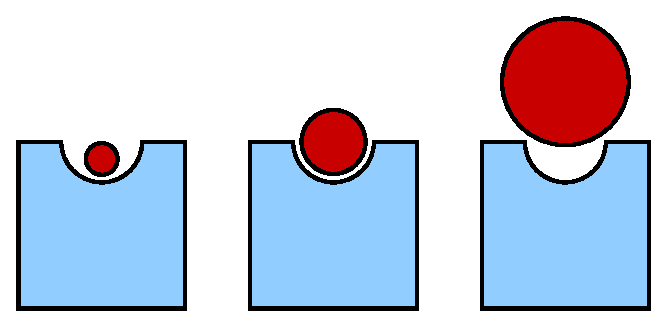
\includegraphics[width=\textwidth]{fig/binding-pocket}
		\caption{Binding-pocket size}
		\label{fig:pocket-size}
	\end{subfigure}
	\begin{subfigure}[b]{0.45 \textwidth}
		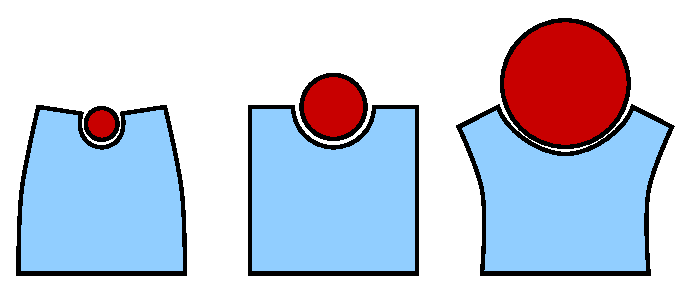
\includegraphics[width=\textwidth]{fig/binding-pocket-flex}
		\caption{Binding-pocket flexibility}
		\label{fig:pocket-flex}
	\end{subfigure}
	\caption{This figure shows different scenarios that may happen when an odorant molecule binds to a receptor. 
	Figure \ref{fig:pocket-size} shows the effect of binding-pocket size. 
	From left to right, misfit because of small size of molecule, perfect match and misfit because of large size of the molecule.
	Figure \ref{fig:pocket-flex} demonstrates that the flexibility of a receptor may compensate the size mismatches. 
	The red disk (dark grey in b\&w) demonstrate an odorant molecule, 
	and the blue shape (light grey in b\&w) represents an odor-receptor and binding-pocket.}
	\label{fig:binding-pocket}
\end{figure}•

Survival of many species depends on their olfactory system. 
They use it  to search for food, avoid poison, escape from danger, find mate, and bind to their offspring.
An olfactory system detects the chemicals in the surrounding, encodes the results and sends them to the higher area of brain. 

Despite the importance of olfactory system, we know very little about it comparing to other senses, 
for example, 
the molecular basis of olfaction was unknown until the break through by Linda B. Buck and Richard Axel, 
which won them a Nobel Prize in Physiology or Medicine, in 2004.
They showed that olfactory receptors are g-protein coupled receptor (GPCR), 
each receptor neuron expresses only one type of olfactory receptor and
their axons are converging a in few glomeruli of the olfactory bulb. 

It is also known that olfactory systems use a combinatorial code: 
an olfactory receptor receptor can be triggered by different odorant molecules, 
and an odorant molecule can excite different olfactory receptors.  
However, it is not clear that which properties of a molecule affects its smell, 
it is a topic of ongoing researches. 

There are many studies that tries to connect physio-chemical properties of molecules to their perceived smells, 
like the current work, which studies the effect of molecular volume of odorants on the response of olfactory receptors.




it includes many olfactory receptors, 
that are supposed to detect thousands of odorants.


and the 3D structure of olfactory receptors are not available.


The olfactory system of insects are similar to the olfactory system of vertebrates in many ways ... 
They are also differences .... 

Some receptors respond to few molecules, some response to many.

Insects receptors neurons show spontaneos activity of 8 Hz.

Drosophila's olfactory receptors are ionotropic. 
They may be metabotropic.

It is under debate.

They have seven trans-membrane domains. 
They need Or83b to work. 
they may construct a complex that work as a cation channel
or Or83b functions as cation channel and collaborte with Olfactory receptor.

Olfactory receptor are presents in other organs like kindny ans sperms.

one reseptor one neurons.

chemical receptory range.


binding-site, binding cavity, binding pocket.
There are MD studies, 
mutagenesis studies,
heterologus expression studies.

in GPCR odorant interact with helix 2,7
2-58 candidate residues.

Drosophila about 60 receptors, mamals 300-1300 receptors. 

In low concentraiotn the response is narrow. In high concentration the response is broad.

OR67d Pheremone. 
Odor prediciton from the shape.
Olfactory white.



\section{Methods}
\begin{figure}
	\centering
	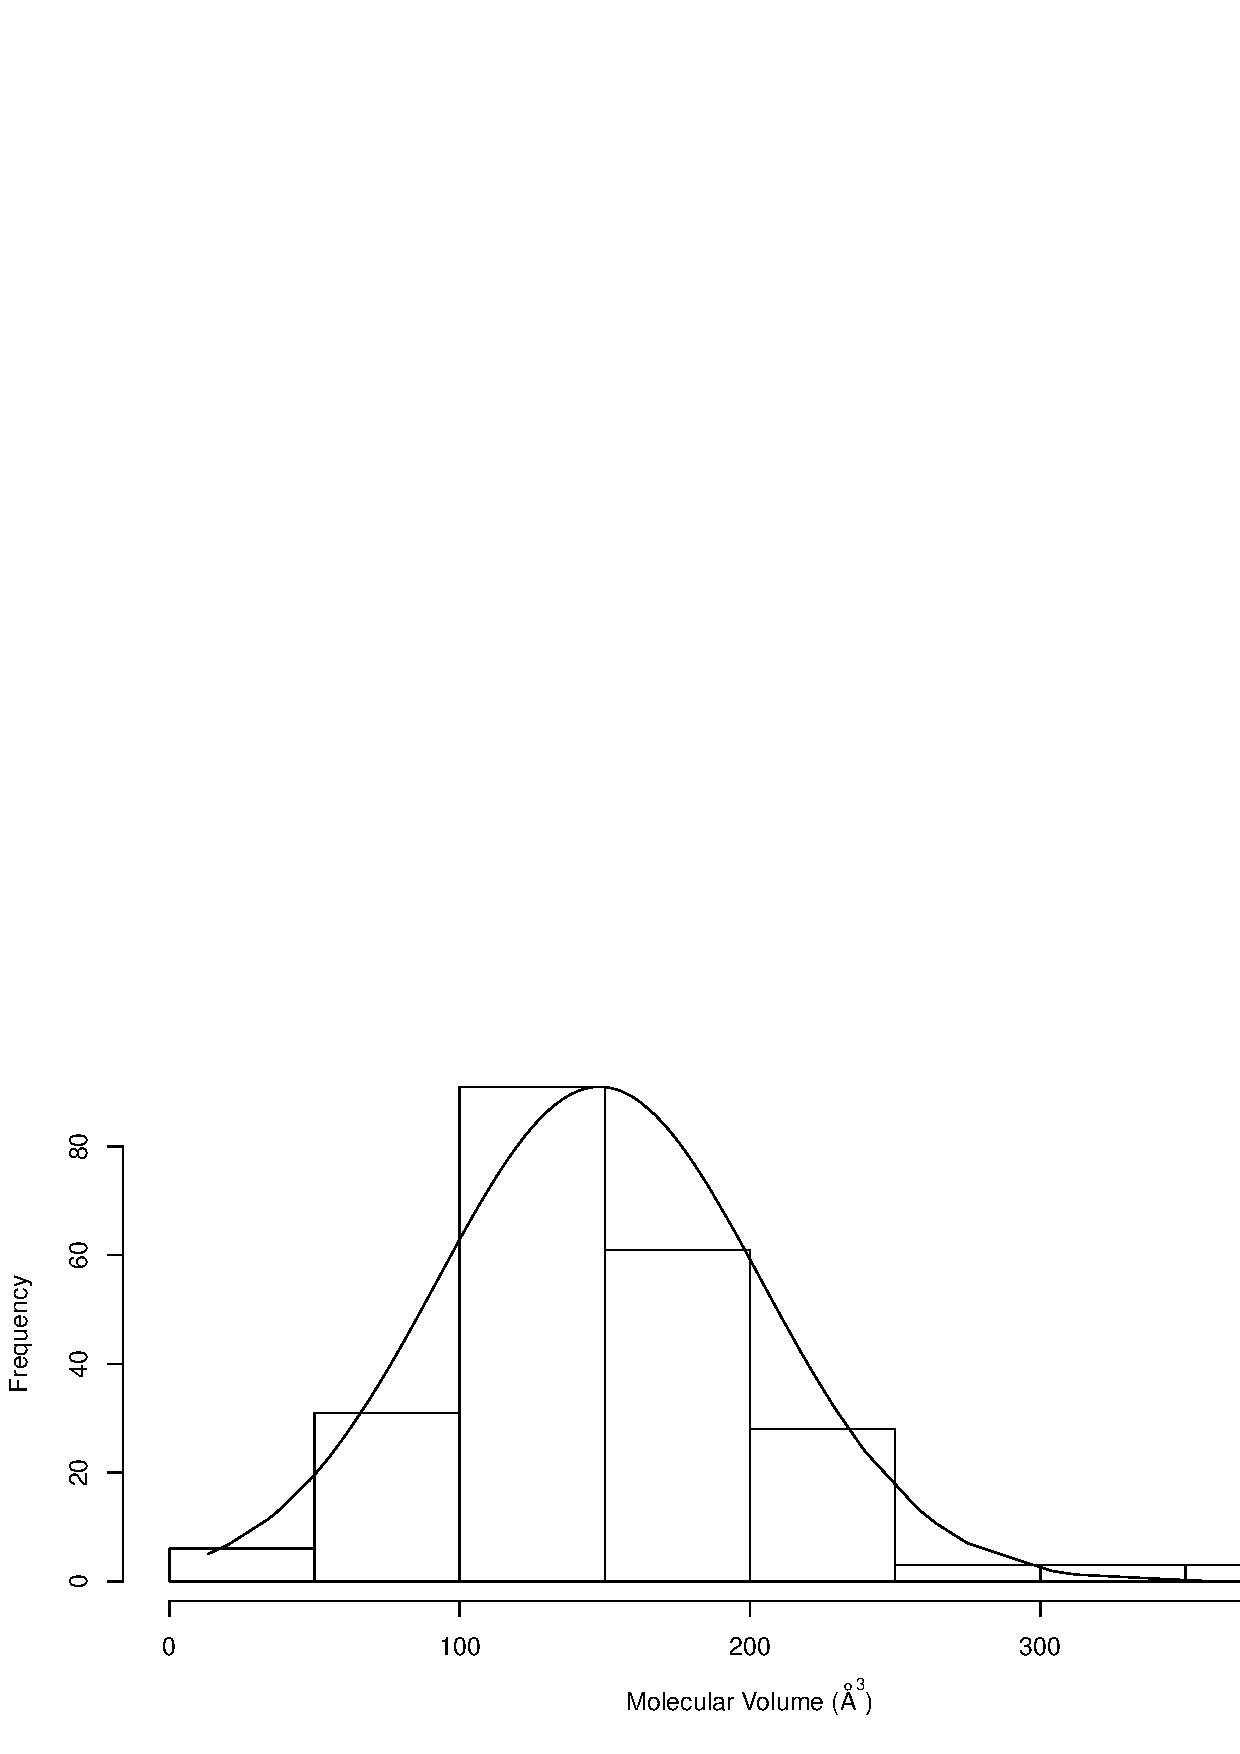
\includegraphics[width=0.5 \textwidth]{fig/hist-volumes}
	\caption{Density function of molecular volumes ($g(v)$), considering all molecules. 
		The actual density function of molecular of volumes in each experiment ($g_n(v)$) might be slightly different 
		because each experiment uses a different subset of molecules. 
		The solid line is a Gaussian fit (Eq. \ref{eqn:hist-volumes}).}
	\label{fig:hist-volumes}
\end{figure}•
We want to study the relation between neural responses and molecular volumes, so we need the respective data. 
We take the neural data of DoOR database \cite{DoOR2010} and we calculate molecular volume using a computational chemistry software -- VEGA ZZ. 

An olfactory receptor neuron $n$ is excited by odorants $m \in M_n$ and the response of $r_{nm}$ is recorded, 
where $0 \le r_{nm} \le 1$. 
Different neurons might be excited by different set of odorants $M_n$. 
The response $r_{nm}$ depends on the molecular volume of the odorant, $v_m$, 
and many other possible physio-chemical properties of the molecule $m$; 
Therefore, we separate the response $r_{nm}$ into two terms:
\begin{equation}
	r_{nm} = f_n(v_m) \psi_{nm}.
	\label{eqn:factors}
\end{equation}
The first term, $f_n(v)$, depends only on the molecular volume of odorants.
The second term, $\psi_{nm}$ may include every other properties of molecules, but the molecular volume.
Both terms are characteristic of each receptor, and they might vary from neuron to neuron.
In fact, the first term, $f_n(v)$, is the tuning curve of neuron $n$ in respect to the feature of molecular volumes, 
and like many other tuning curves, it can be approximated with a Gaussian function
\begin{equation}
	\displaystyle f_n(v) = e^{-\frac{(v-v_n)^2}{2\sigma^2_n}}, 
	\label{eqn:volume-dependence}
\end{equation}
where, $v_n$ is the preferred molecular volume of receptor $n$ and $\sigma_n$ represents its volume selectivity. 
In this work we want to estimate $v_n$ and $\sigma_n$. 
To do so, first we calculate the response weighted average of molecular volumes, 
$\frac{\sum_{m\in M_n} v_m r_{nm}}{\sum_{m\in M_n} r_{nm}}$ and then we use equation \ref{eqn:factors}:
\begin{equation}
	\frac{\displaystyle \sum_{m\in M_n} v_m r_{nm}}{\displaystyle \sum_{m\in M_n} r_{nm}} = \frac{\displaystyle \sum_{m\in M_n} v_m f_n(v_m) \psi_{nm}}{\displaystyle \sum_{m\in M_n} f_n(v_m) \psi_{nm}}.
	\label{eqn:sta}
\end{equation}
Here we can convert $\sum$ to $\int$ following this rule:
\begin{equation}
	\sum_{m\in M_n} \dots f_n(v_m) \psi_{nm} =  \langle \psi_{nm} \rangle_m \int_0^\infty \dots f_n(v) g_n(v)  dv. 
	\label{eqn:sigma_to_int}
\end{equation}
In which, 
$\langle \psi_{nm} \rangle_m$ denotes the average of $\psi_{nm}$ over all $m \in M_n$, 
and can be moved out of the integral for it is independent of $v$.
In the above equation, 
$g_n(v)$ is the density of states, it says for each set of odorants $M_n$, how many molecules have a molecular volume in the range of $v$ and $v+dv$.
This function can be approximated by a Gaussian function of the form (Fig.\ref{fig:hist-volumes})
\begin{equation}
	g_n(v) = e^{-\frac{(v- v_{M_n})^2}{2\sigma_{M_n}^2}},
	\label{eqn:hist-volumes}
\end{equation}
where $v_{M_n}$ and $\sigma_{M_n}$ are the average and standard deviation of molecular volume of the set $M_n$.
Now we convert $\sum$ to $\int$ in equation \ref{eqn:sta} using equation \ref{eqn:sigma_to_int}, to get
\begin{equation}
	\frac{\displaystyle \sum_{m\in M_n} v_m r_{nm}}{\displaystyle \sum_{m\in M_n} r_{nm}} = \frac{\displaystyle \int v f_n(v) g_n(v) dv}{\displaystyle \int f_n(v) g_n(v) dv}.
	\label{eqn:sta_int}
\end{equation}
We replace the product of $f_n(v)$ and $g_n(v)$ in the above equation with $h_n(v) = f_n(v) g_n(v)$, to make a simpler form
\begin{equation}
	\frac{\displaystyle \sum_{m\in M_n} v_m r_{nm}}{\displaystyle \sum_{m\in M_n} r_{nm}} = \frac{\displaystyle \int_v v h_n(v) dv}{ \displaystyle \int_v  h_n(v) dv }.
	\label{eqn:mean}
\end{equation}
The function $h_n(v)$ is a Gaussian function because it is the product of two Gaussian functions, 
\begin{equation}
h_n(v) = e^{-\frac{(v-\mu_{h_n})^2}{2\sigma_{h_n}^2}}, 
\end{equation}
so the right hand side of equation \ref{eqn:mean} is nothing but $\mu_{h_n}$. 
In a similar way, we can calculate $\sigma_{h_n}$ from the neural data.

We knew the mean $v_{M_n}$ and standard deviation $\sigma_{M_n}$ of $g_n(v)$ from the properties of the molecules. 
We just calculated the mean $\mu_{h_n}$ and standard deviation $\sigma_{h_n}$ of $h_n(v)$ from the neural data.
Now calculating the mean $v_n$ and the standard deviation $\sigma_n$ of $f_n(v)$ is trivial,
first we calculate $\sigma_n$ from 
\begin{equation}
	\sigma_n^2 = \frac{\sigma^2_{g_n} \sigma^2_{h_n}}{\sigma^2_{g_n} - \sigma^2_{h_n}}
\end{equation}•
and then we calculate $v_n$ from 
\begin{equation}
	v_n =  \sigma_n^2 \left ( \frac{\mu_{h_n}}{\sigma^2_{h_n}} - \frac{v_{g_n}}{\sigma^2_{g_n}} \right ).
\end{equation}•
The resulting $f_n(v)$ are plotted over the actual data, for one receptor and for all 28 receptors (Fig.~\ref{fig:vol-res}).
Now we know the preferred volume $v_n$ of each receptor and also its volume selectivity $\sigma_n$.


\section{Results}
\begin{figure}
	\centering
	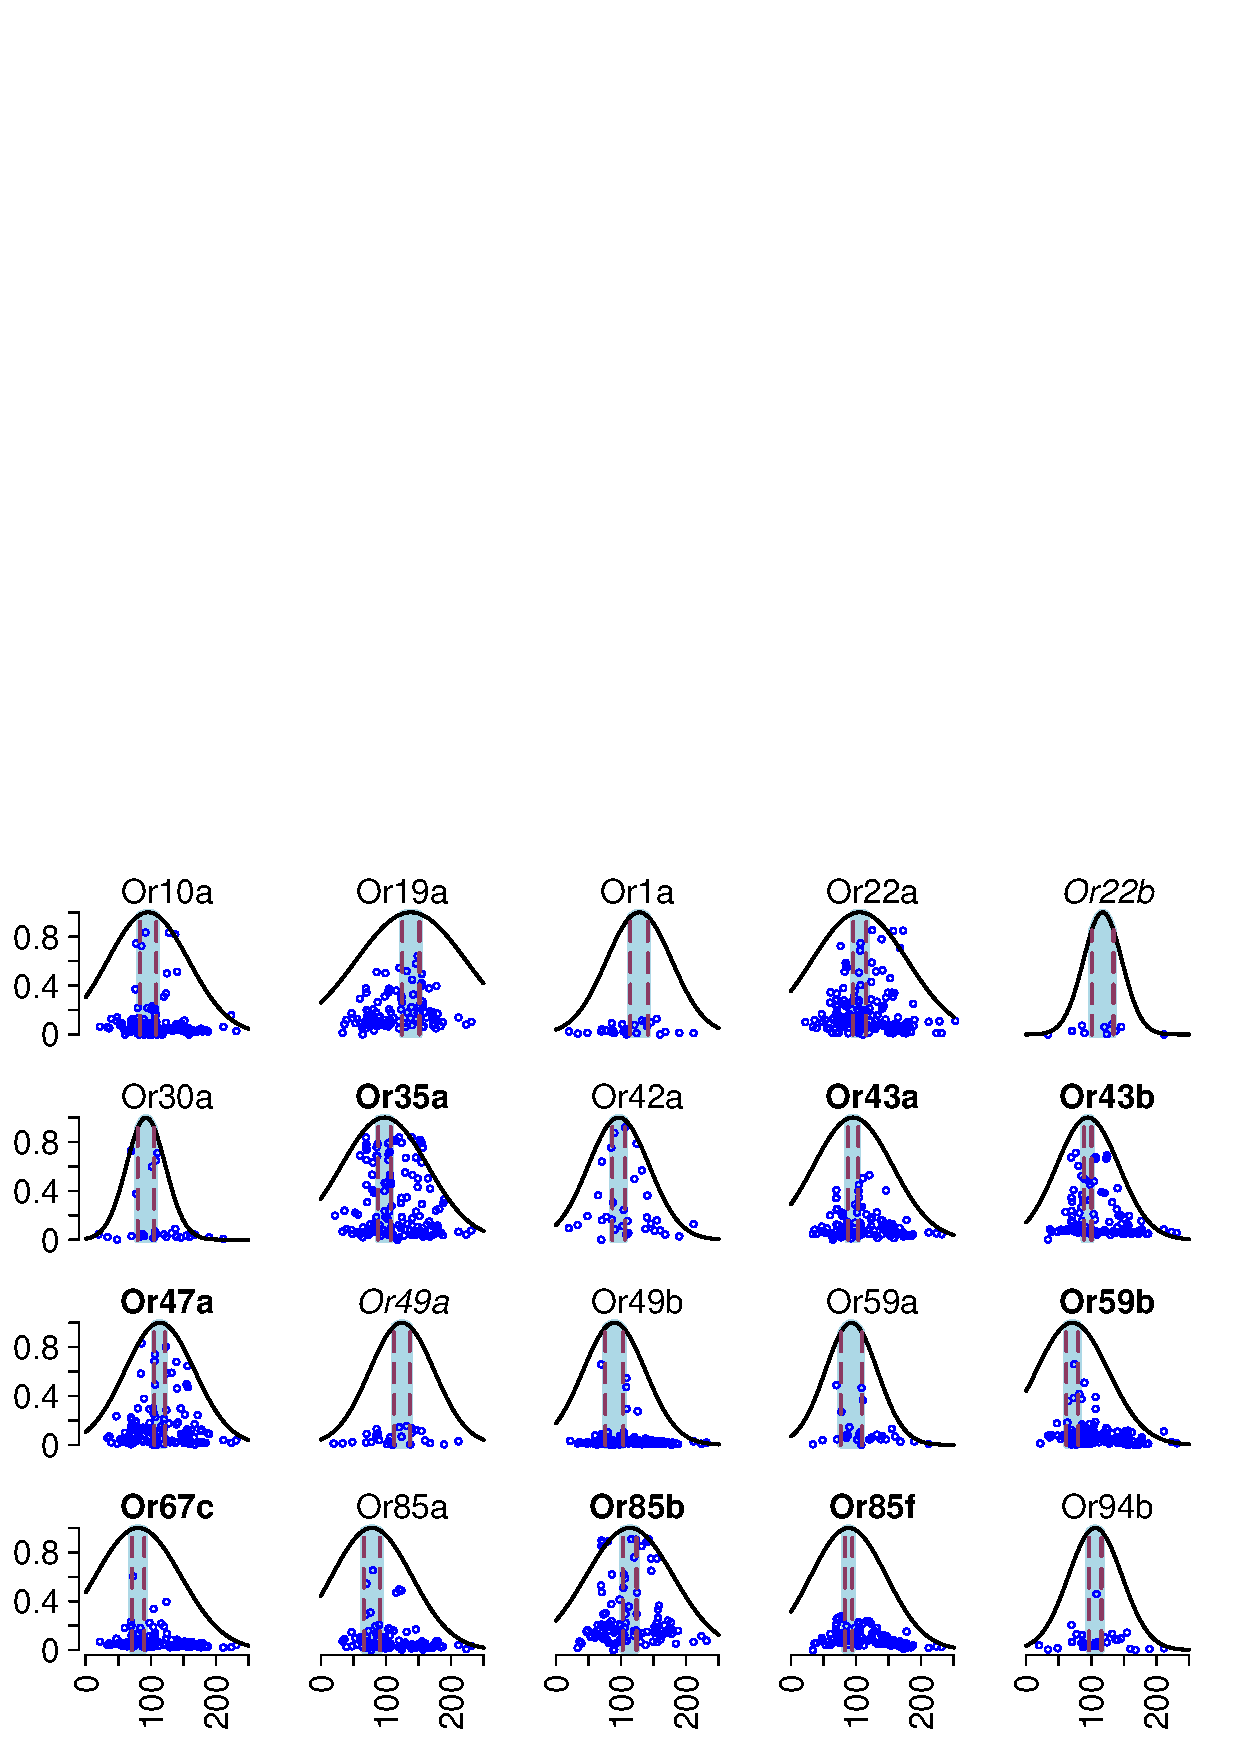
\includegraphics[width=\textwidth]{fig/vol-res}
	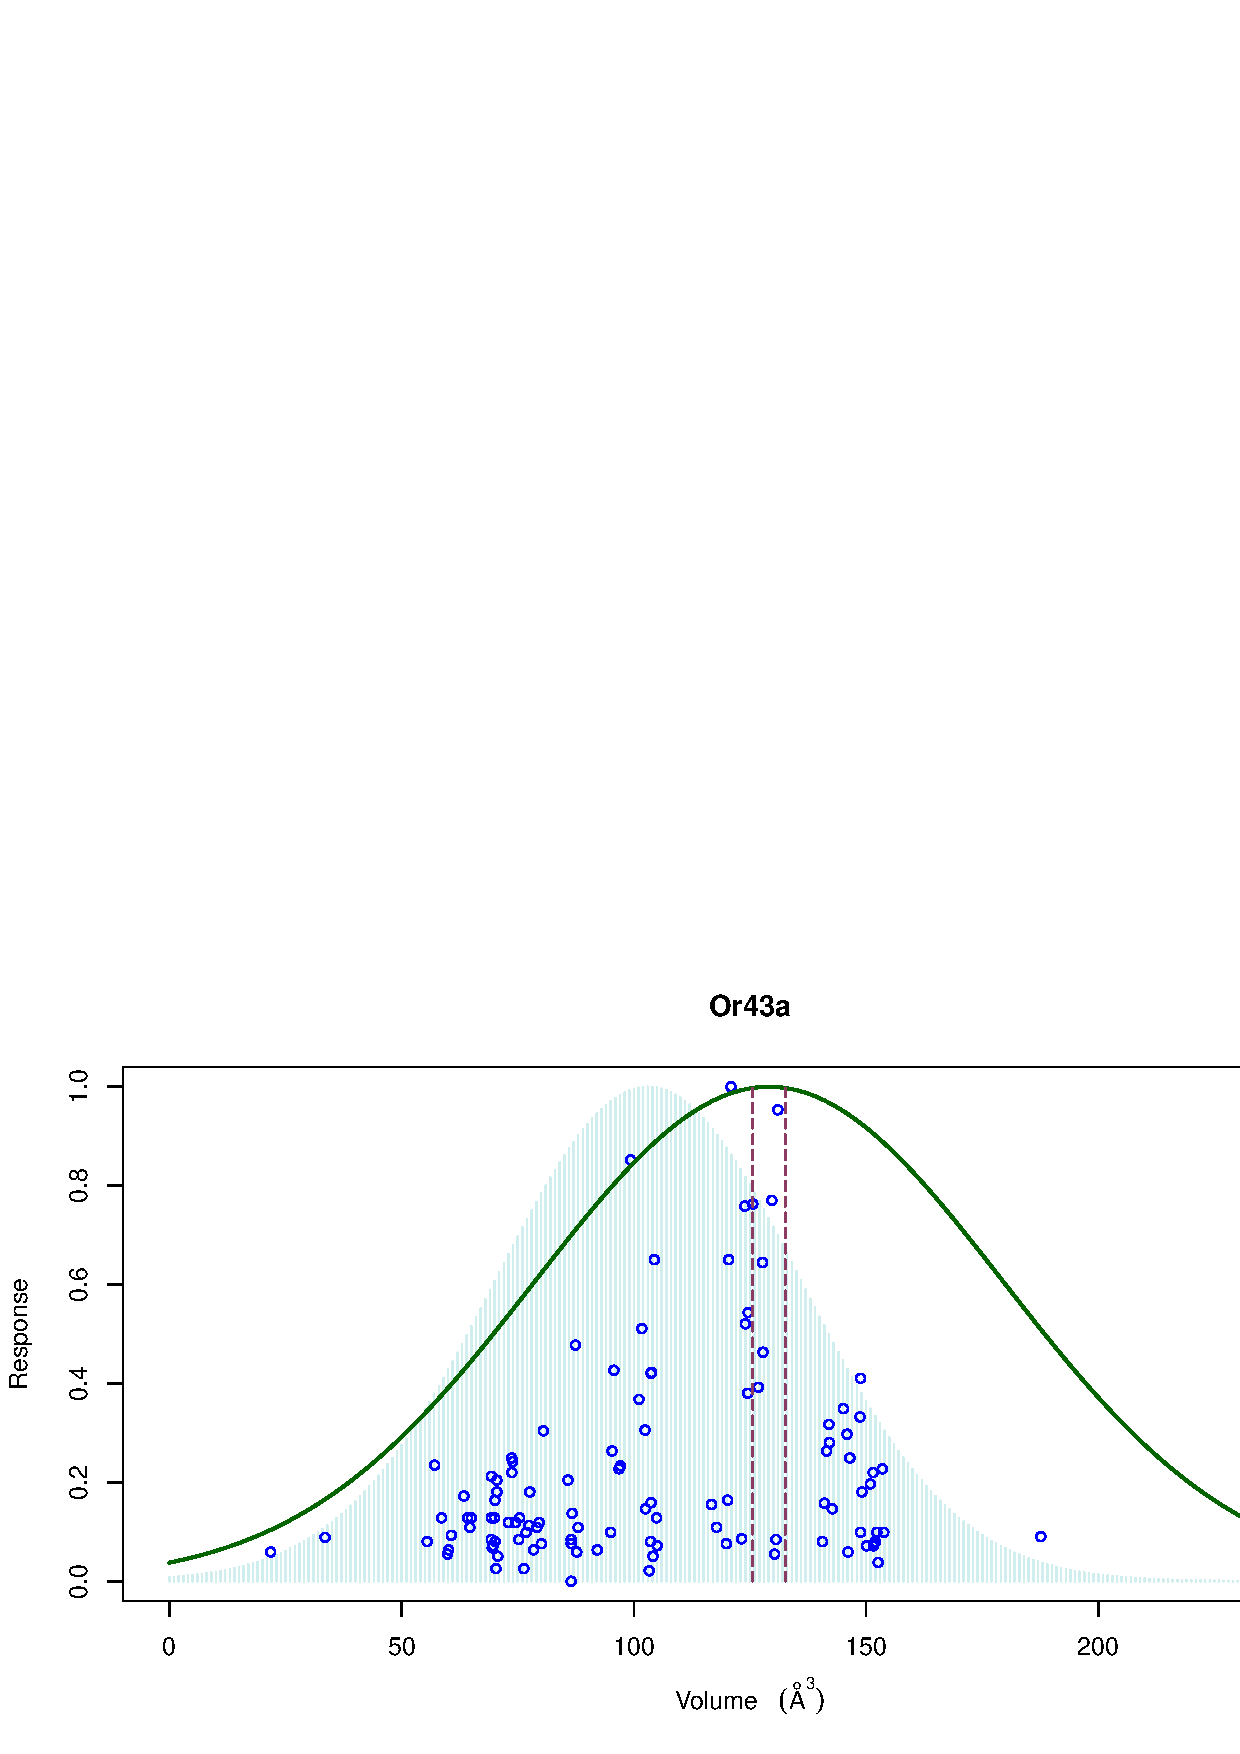
\includegraphics[width=0.75 \textwidth]{fig/vol-res-Or42a}
	\caption{Response of odor-receptors  versus molecular volume of odorants (Circles), and the fitted functions $f_n(v)$ from Eq. \ref{eqn:factors} (solid lines), 
	for all 28 receptors (top) and for one selected receptor Or42a(bottom) to demonstrate the details. }
	\label{fig:vol-res}
\end{figure}•

\begin{figure}
	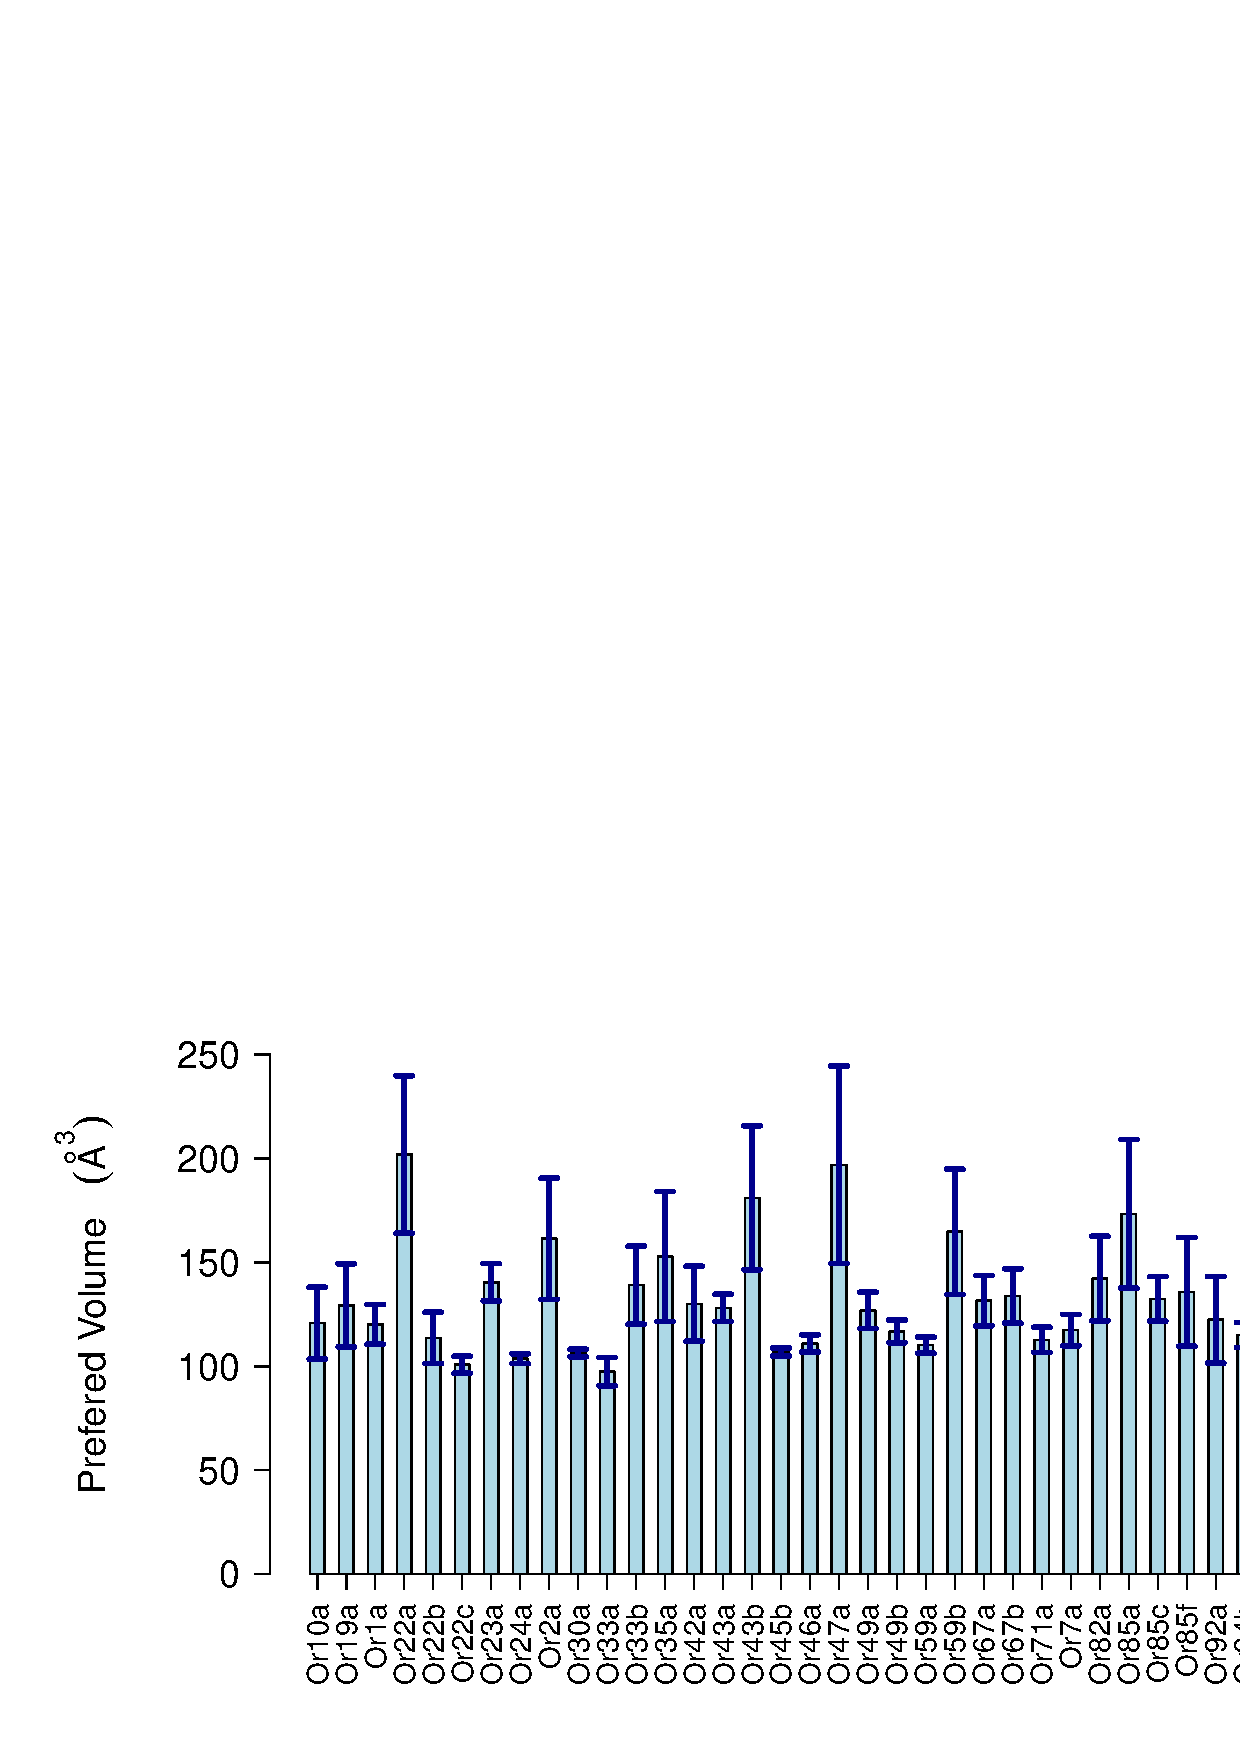
\includegraphics[width=\textwidth]{fig/mean-vol}
	\caption{The prefered volumes of 28 receptors ($v_n$), and their error bars. Error bars are calculated using Jack-Knife method. 
	This figure suggests that the size of binding-pocket varies across receptors. 
	Some receptors binds to smaller molecules (Or52b) but some other receptors prefer larger molecules (Or13a and Or98a).}
	\label{fig:preferred_volume}
\end{figure}•

\begin{figure}
	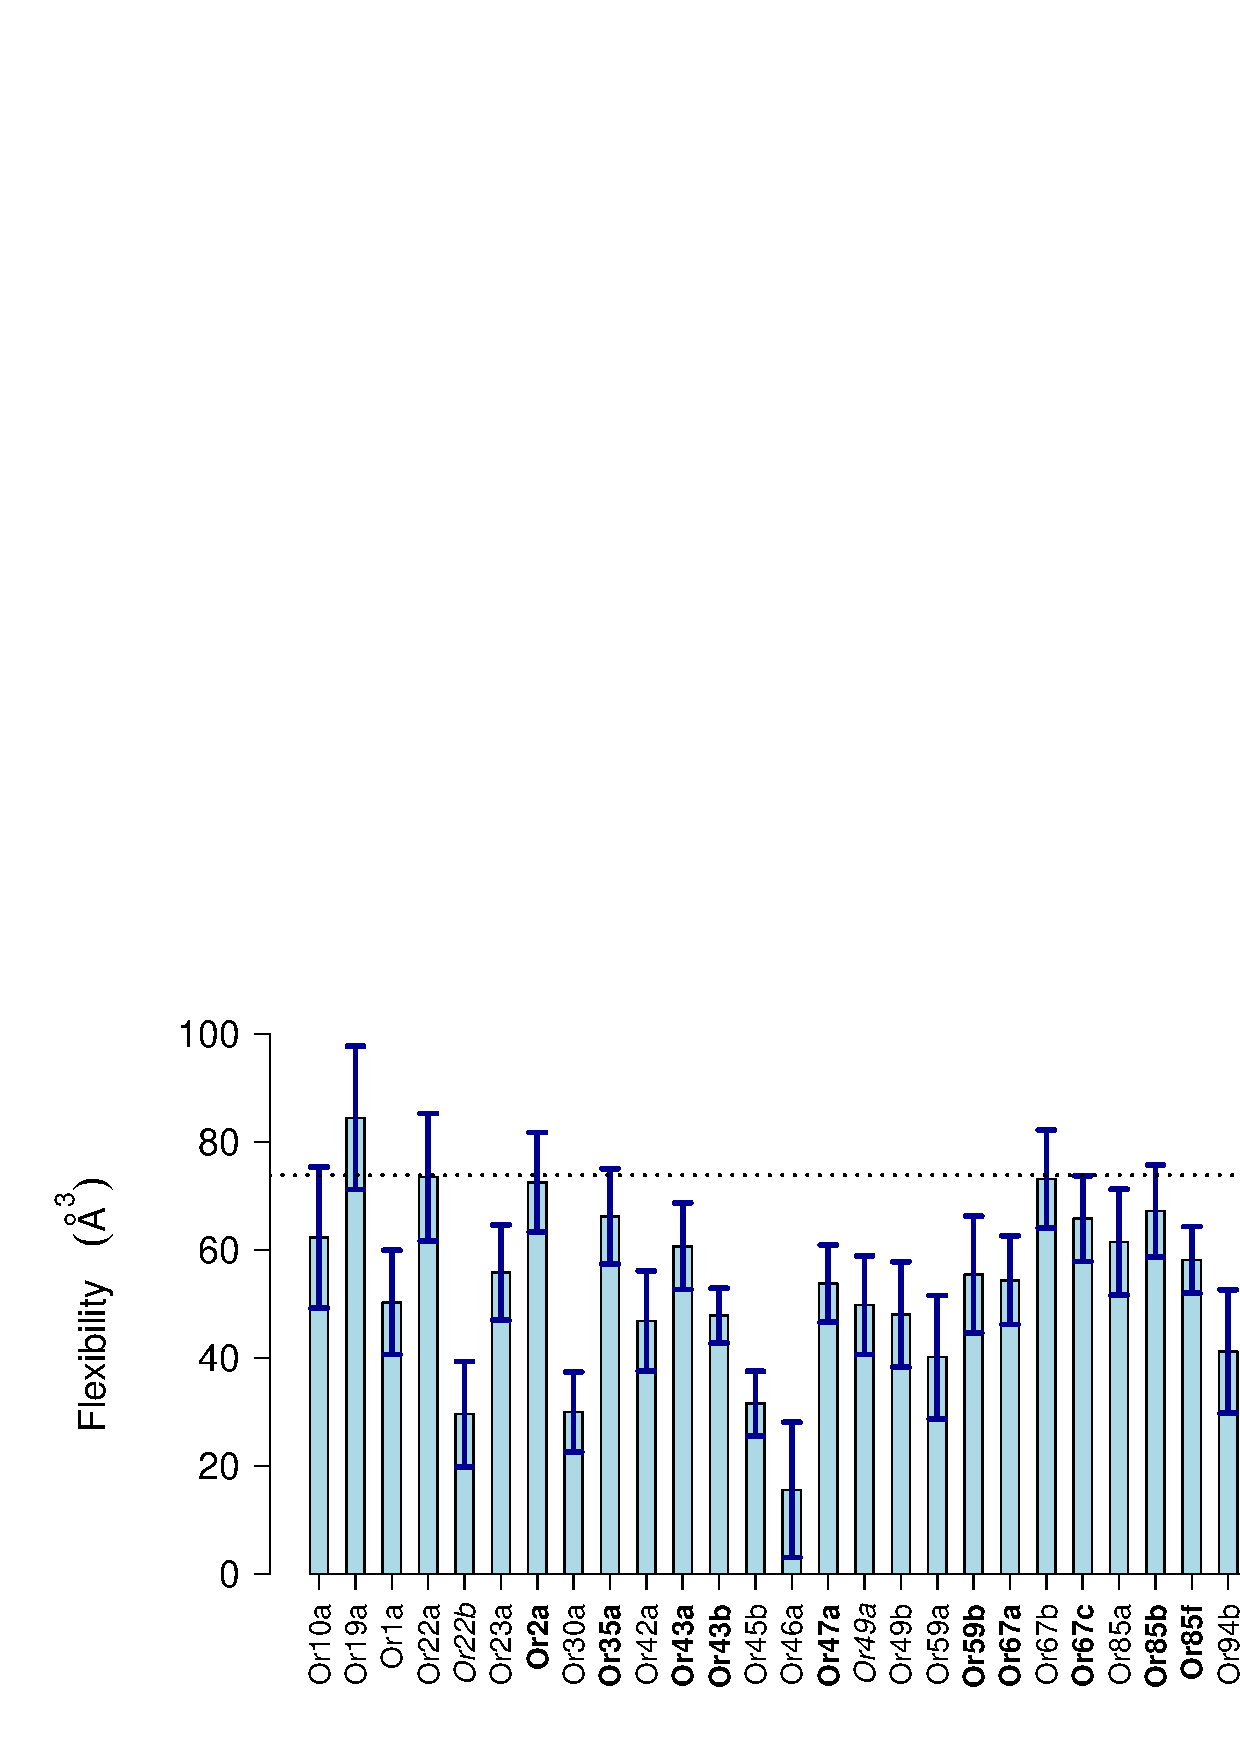
\includegraphics[width=\textwidth]{fig/std-vol}
	\caption{This figure shows the volume selectivity of each receptor ($\sigma_n$), the error bars are calculated using Jack-Knife method.
	Some receptors like Or30a are more volume selective but on the other hand, some other receptors like Or13a and Or42b are less sensitive toward the molecular volumes.
	This might be due to mechanical flexibility of the binding-pocket.}
	\label{fig:volume_selectivity}
\end{figure}•

The function $f_n(v)$ can be considered as the tuning curve of olfactory receptors in response to molecular volume;
Therefore, each receptor has a preferred molecular volume $v_n$ and receptors can show different degree of selectivity $\sigma_n$.
We calculated the parameters of $f_n(v)$ for 28 receptors (Fig. \ref{fig:vol-res}). 
The calculated values, $v_n$ and $\sigma_n$ are in Fig. \ref{fig:preferred_volume} and \ref{fig:volume_selectivity} respectively.
Figure \ref{fig:preferred_volume} demonstrate that the molecular volume preference of receptors are different. 
Figure \ref{fig:volume_selectivity} illustrate that the volume selectivity of receptors are also different.

It is not clear which features of molecules are measured by olfactory receptors, yet. 
It is a topic of ongoing researches 
and there are many works that tries to make connections between physio-chemical properties of molecule 
and the evoked neural response. 
But this non-linear volume dependence (Eq. \ref{eqn:factors} and Eq. \ref{eqn:volume-dependence}) is in the way. 
It may mask important relations between molecules and neural responses.

By considering our finding and correcting the effect of molecular volume on the response of olfactory receptor neurons, 
one might discover more subtle dependence between molecular features and neural responses, 
which otherwise would be masked by this non-linear effect.

We also make some prediction about the 3D structure of olfactory receptors:
The preferred volume of each receptor results from the size of the binding-pocket; 
The volume selectivity of a receptor results from the rigidity or flexibility of the binding-pocket; 
Therefore, our results provides information about both structural and dynamical properties of olfactory receptors in Drosophila. 
These data add some constrains over the 3D structure of olfactory receptors, 
which may help the prediction or calculation of the 3D structure of these proteins. 

The method of this work can be combined with mutagenesis as well. 
Some genes of an olfactory receptor are mutated, 
then its response to a selection of molecules are measured and finally the preferred volume and volume selectivity are calculated.
In this way we can understand which amino acids of the olfactory receptor contribute to the size and flexibility of the binding-pocket, 
as well as affecting the function of the receptors.

In this work we studied the factor $f_n(v)$ of the equation \ref{eqn:factors} and we said nothing about $\psi_{nm}$. 
To study $\psi_{nm}$, more data are necessary. 
To save time and expenses of the experiments, 
it is better if these additional data were around the preferred volume of each olfactory receptor.
In table \ref{tab:receptor-odorant} we suggested the best selection of odorants for each of 28 studied receptors.

\begin{table}
	\begin{tabular}{|l|l|l|}
		\hline 
		Olfactory receptor & studied odorants & proposed odorants \\ \hline 
		OrXa & 
	\end{tabular}
	\caption{I have to think to the layout ...}
	\label{tab:receptor-odorant}
\end{table}•

\bibliographystyle{plain}
\bibliography{binding-pocket}

\end{document}
